\documentclass[11pt]{article}
\usepackage[utf8]{inputenc}
\usepackage[T1]{fontenc}
\usepackage[french]{babel}
\usepackage{listings}
\usepackage{geometry}
\usepackage{hyperref}
\usepackage{fancyhdr}
\usepackage{graphicx}

\geometry{margin=2.5cm, vmargin=2.5cm}
\pagestyle{fancy}
\fancyhf{}
\graphicspath{screens yan/}

\title{RAPPORT PROJET CDAA}
\author{Yann TROU | TD2 Groupe B}
\date{Octobre 2020}

\begin{document}

\maketitle
\tableofcontents
    
    \vspace{\baselineskip}
    \vspace{\baselineskip}
    
    \chapter{\large{I | Cahier des charges}}
    \begin{center}
        \subsection*{1. Fonctions}
        \subsection*{2. Structures}
    \vspace{\baselineskip}
    \vspace{\baselineskip}
    \end{center}
    
    \chapter{\large\texitit{II | Analyse fonctionnelle}} \\
    
    \begin{center}
        \subsection*{1. Classes et packages}
        \subsection*{2. Affichage et CLI}
        \subsection*{3. Interactions et commandes}
    \end{center}
    
    \chapter{\Large\texitit{III | Manuel d'utilisation}}
    
    \begin{center}
        \subsection*{1. Commandes}
        \subsection*{2. Dépannage}
    \end{center}
    
    \chapter{\Large\texitit{IV | Panier d'objets génériques}}
    
\newpage
\fancyhf{}
\lhead{I | Cahier des charges}
\lfoot{Page \thepage}
    \section*{I | Cahier des charges}
    \subsection*{1. Fonctions}
\\
On peut définir le cahier des charges à partir des sujets de TP et TD en plus de l'énoncé du sujet.\\
L'objectif est pour le moment de créer un prototype de site de vente de jeux vidéos, consoles, et autres.
Ce prototype se limitera à la ligne de commande pour l'interface et de la gestion de catalogue. Le sujet indique que l'on doit ajouter un autre type d'objets gérés en plus des jeux. J'ai choisi des Consoles.
Ainsi, les fonctionnalités attendues sont:
    \begin{itemize}
        \item Ajouter un jeu / une console
        \item Supprimer un jeu / une console
        \item Visualiser tous les jeux / toutes les consoles
        \item Rechercher dans les jeux ou les consoles avec des paramètres spécifiques
        \item Trier les jeux ou les consoles par champ
        \item Pouvoir gérer des jeux rétro
    \end{itemize}

    \subsection*{2. Structures}
\\
Les structures de données proposées par le tp sont les suivantes: un catalogue regroupant les ensembles d'objets vendables, ces mêmes ensembles utilisant List<> pour stocker leurs éléments. Ensemble est une classe abstraite regroupant des méthodes pour ajouter, supprimer, trier et rechercher. Les implémentations de cette classe sont EnsembleJeux et EnsembleConsoles respectivement pour les jeux et les consoles.

\newpage{}
\fancyhf{}
\lhead{II | Analyse Fonctionnelle}
\lfoot{Page \thepage}

    \section*{II | Analyse Fonctionnelle}
    Faute de pouvoir le faire tenir dans ce fichier pdf, le graphique détaillé des classes, packages et relations se trouve en annexe dans le fichier DiagrammeClasses.jpg. 
    
    \subsection*{1. Classes et packages}
    \\
    A partir du cahier des charges, nous pouvons commencer à définir les grandes lignes de notre programme.
    Nous aurons besoin d'un ensemble de classes représentant les jeux et les consoles, un package contenant les structures de données, un package pour l'application des commandes.
    \\\\
    Pour les jeux nous aurons donc: 
    \begin{itemize}
        \item une classe Jeu pour représenter un jeu
        \item une classe JeuRetro héritant de Jeu pour représenter un jeu rétro 
        \item une énumération Genre pour indiquer le genre de jeu
        \item une classe EnsembleJeu qui hérite de Ensemble et se spécialise pour gérer des jeux.
    \end{itemize}
    \vspace{\baselineskip}
    Pour les consoles nous aurons un jeu de classes similaires
    \\
    Nous aurons une classe Catalogue qui contiendra un ensemble de chaque produit et servira de point d'accès vers ceux-ci
    \\
    Pour pouvoir trier ces objets, nous allons utiliser un tri quicksort dans la classe du même nom. 
    \\
    Afin de pouvoir spécifier l'attribut sur lequel trier les objets, on va créer une interface IFieldComparable avec une seule méthode, CompareFieldTo. l'implémentation de cette méthode sera faite dans les classes Jeu et Console.
    \\
    Pour pouvoir faire des ensembles d'objets, il nous faut la classe abstraite ensemble
    \\
    Il nout faut aussi une classe permettant de faire interagir toutes ces autres classes, ce sera le rôle de la classe Program.
    \\
    Enfin, les classes CommandesConsoles et CommandesJeux serviront à séparer les implémentations des commandes de la classe Program pour l'alléger.
    \\\\
    Nous pouvons en déduire les packages suivants:
    \begin{itemize}
        \item CLI : classes liées à l'affichage dans la console
        \item commands : classes pour traiter les commandes
        \item Core : noyau du programme
        \begin{itemize}
            \item consoles : classes liées à la représentation d'une console
            \item jeux : classes liées à la représentation d'un jeu
        \end{itemize}
        \item datastructures : structures de données génériques utilisées dans d'autres parties du programme
        \item doc : fichiers texte ayant servi à l'élaboration du programme
    \end{itemize}
    
    \subsection*{2. Affichage et CLI}
    \\
    Pour plus de confort et de lisibilité, j'ai eu l'idée d'implémenter un système d'affichage dans la console se contrôlant au clavier et reprennant des éléments similaires à ceux que l'on peut trouver dans de vrai programmes avec une interface. 
    \\\\
    Maintenant, pour le traitement et l'affichage, je me suis inspiré de \href{https://www.youtube.com/watch?v=jde1Jq5dF0E}{ cette vidéo (cliquez)}. Les principaux éléments que j'ai retenu sont l'utilisation d'une pile pour stocker et afficher avec de la profondeur les éléments d'interface et aussi le fait que les éléments se dessinent eux mêmes. L'utilisation d'une pile permet de ne donner le contrôle qu'a un seul élément, celui tout en haut de la pile donc au premier plan. 
    \\\\
    La différence principale tient au fait que la où il a un moteur pour afficher des images en couleur, je n'ai que la console. Mais heureusement, la console possède une méthode SetCursorPosition, permettant de placer le curseur n'importe ou dans les limites de la fenêtre et d'écrire ce que l'on veut. Nous avons les bases du système de CLI.
    \\\\
    J'ai pour commencer crée la classe CLIManager, qui contient et gère la pile de CLIElement, classe mère de tous les éléments. CLIManager ne contient pas grand chose, des méthodes pour ajouter et supprimer des CLIElement, une méthode pour mettre a jour l'affichage et une méthode Loop. Cette méthode est importante car c'est la boucle principale du programme: mettre à jour le contenu de la table, mettre à jour l'affichage, récupérer la touche que l'utilisateur a pressé et la transmettre à l'élément en haut du tas, et recommencer.
    \\\\
    Maintenant, parlons des éléments d'interface disponibles et de leurs classes.
    \\
    Les éléments qui ont été implémentés sont
    \begin{itemize}
        \item une fenêtre vide : classe CLIWindow. au final il ne s'agit que d'une bordure
        \item une fenêtre modale : classe CLIInputWindow. permet à l'utilisateur de rentrer du texte, et de le récupérer dans le programme
        \item un menu (vu comme une liste) : classe CLIMenu. permet de parcourir des commandes et d'en séléctionner une.
        \item un tableau : classe CLITable. permet d'afficher sous forme de table des données. 
    \end{itemize}
    \vspace{\baselineskip}
    \\\\
    L'un des problèmes que j'ai rencontré est la vitesse d'affichage. En effet, à un point on voyait tous les éléments se dessiner plutôt que l'affichage soit fait instantanément. Une première solution a été de concaténer des chaines de caractères en une seule pour réduire le nombre d'appels  à SetCursorPosition et Write mais aussi de supprimer les boucles d'affichage horizontal. Mais cette solution a été remplacée par l'utilisation de StringBuilder. Car, après un tour dans la documentation microsoft \href{https://docs.microsoft.com/fr-fr/dotnet/api/system.string?view=netcore-3.1}{(ici précisément)} j'ai appris que les strings étaient immutables et qu'a chaque opération, ils étaient copiés et l'opération était appliquée sur la copie. De plus, le fait que la méthode Append() puisse ajouter n fois un caractère permet d'optimiser encore mieux le code. Avec tout cela, nous avons retrouvé des vitesses d'affichage quasiment instantanées. 
    \\\\
    Un des problèmes récurrent et que vous pouvez recontrer, tient du fait que la taille de la console varie en fonction de chaque écran et de chaque résolution et des erreurs dues à des débordement peuvent apparaitre. Dans certains cas, la console n'est pas du tout supportée (comme sur mon mac).
    Si le programme ne fonctionne pas, s'il vous plait jetez un coup d'oeil au manuel ou au pire contactez moi.

    \section*{3. Interactions et commandes}
    Ici, nous allons détailler comment les commandes sont traitées.
    \\
    Déjà, chaque commande est identifiée par un entier. Elles ont été définies en amont du codage et sont réparties ainsi:
    \begin{itemize}
        \item de -infini à  -1 : commandes générales
        \begin{itemize}
            \item -1 : suppression de la recherche et affichage de toute la table des jeux
            \item -2 : suppression de la recherche et affichage de toute la table des consoles.
        \end{itemize}
        \item de 0 à 99 : commandes pour les jeux
        \begin{itemize}
            \item 0 : ajouter un jeu
            \item 1 : supprimer un jeu
            \item 2 : trier les jeux
            \item 3 : faire une recherche dans les jeux
            \item de 20 à 27 : chaque commande correspond à un champ sur lequel appliquer le tri
            \item de 30 à 37 : chaque commande correspond à un champ sur lequel appliquer une recherche
        \end{itemize}
        \item de 100 à 199 : commandes pour les consoles
        \begin{itemize}
            \item 100 : ajouter une console
            \item 101 : supprimer une console
            \item 102 : trier les consoles
            \item 103 : rechercher une console
            \item de 120 à 127 : chaque commande correspond à un champ sur lequel appliquer le tri
            \item de 130 à 137 : chaque commande correspond à un champ sur lequel appliquer une recherche
        \end{itemize}
    \end{itemize}
    \vspace{\baselineskip}
    
    Le cycle de vie d'une commande fonctionne ainsi: dans un CLIMenu, l'utilisateur appuie sur entrée. La commande associée à la position du curseur est envoyée à Program via la méthode statique dispatchCommand. Ensuite, en fonction de l'état du programme, soit la commande est traitée dans commandesJeux si l'état du programme est à 0, soit la commande est traitée dans commandesJeux si l'état du programme est à 1. Dans n'importe quel état elle est testée par rapport aux commandes générales. 
    \\
    Les commmandes s'appliquent de manière similaires aux jeux et aux consoles. 
    \\
    Pour ajouter un jeu, on va créer une CLIInputWindow, l'initialiser pour qu'elle ai le message correspondant et la placer dans la pile d'affichage. Ensuite, on met à jour l'affichage, on place l'entrée claver sur celle ci. Une fois que l'utilisateur a rentré du texte, on le récupère, on le cast si nécessaire et on le set dans le jeu. On recommence pour chaque attribut. Une fois qu'ils sont tous rentrés, on supprime la CLIInputWindow de la pile d'affichage et on ajoute le jeu dans le catalogue.
    
\newpage
\fancyhf{}
\lhead{III | Manuel}
\lfoot{Page \thepage}
    \section*{III | Manuel}
    Pour retrouver toutes les images dans leur taille originale, allez voir /doc/Rapport/ dans le dossier du code source du projet.
    \begin{figure}[ht]
        \centering
        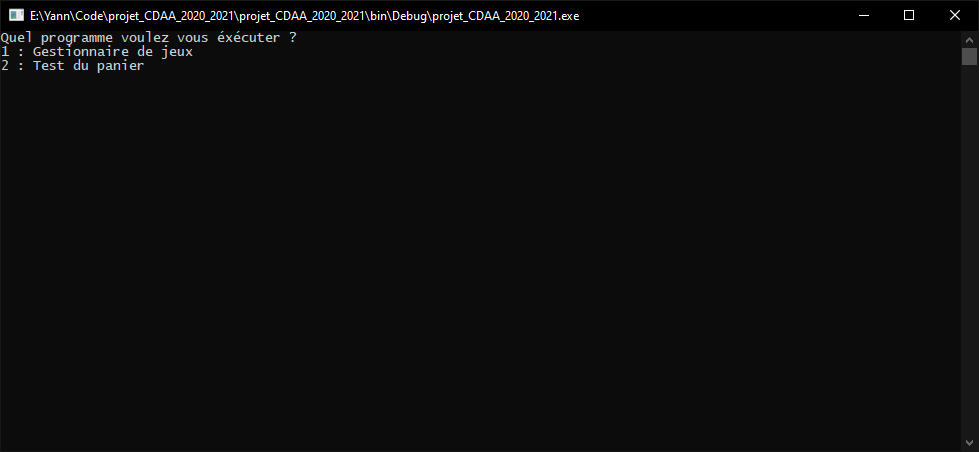
\includegraphics[scale=0.5]{screens yann/ecran1.png}
        \caption{ Lorsque le programme démarre, il vous demande quel programme éxécuter}
        
        \vspace{\baselineskip}
        
        \centering
        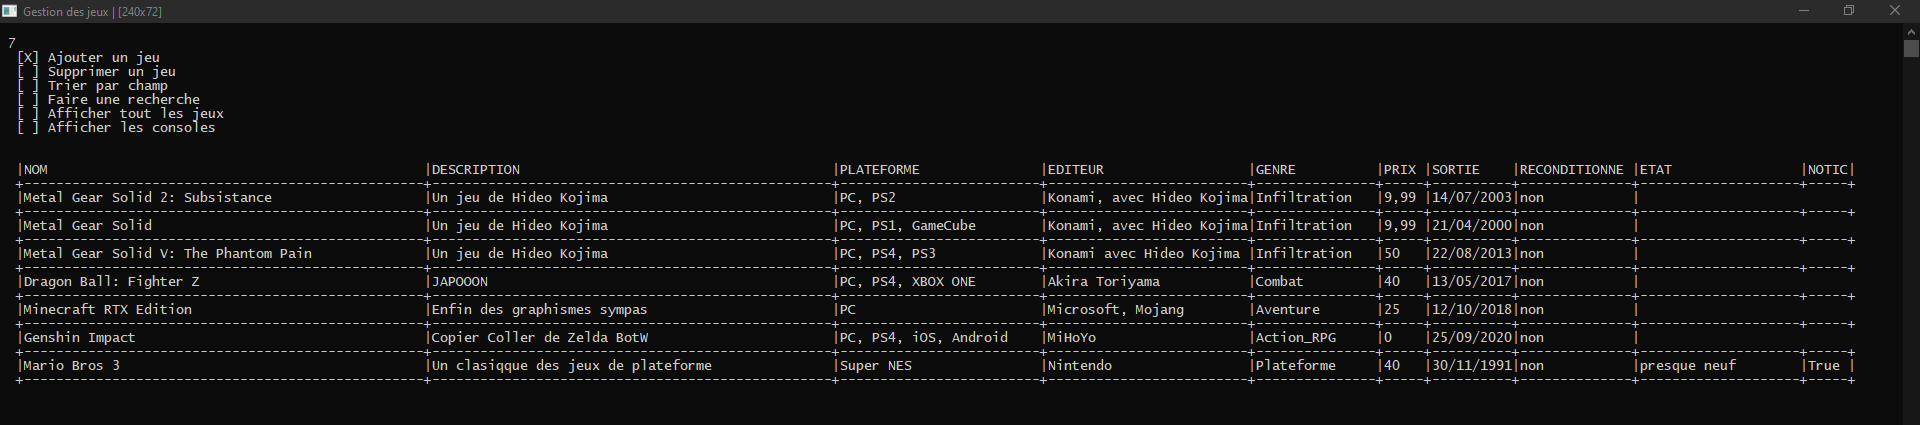
\includegraphics[scale=0.3]{screens yann/ecran_2_main_gest_jeux.png}
        \caption{On peut voir le menu pour la séléction des commandes ainsi que la table qui affiche tous les jeux. Pour se déplacer dans le menu, on utilise les flèches haut et bas et entrée pour séléctionner une commande}
        
        \vspace{\baselineskip}
        
        \centering
        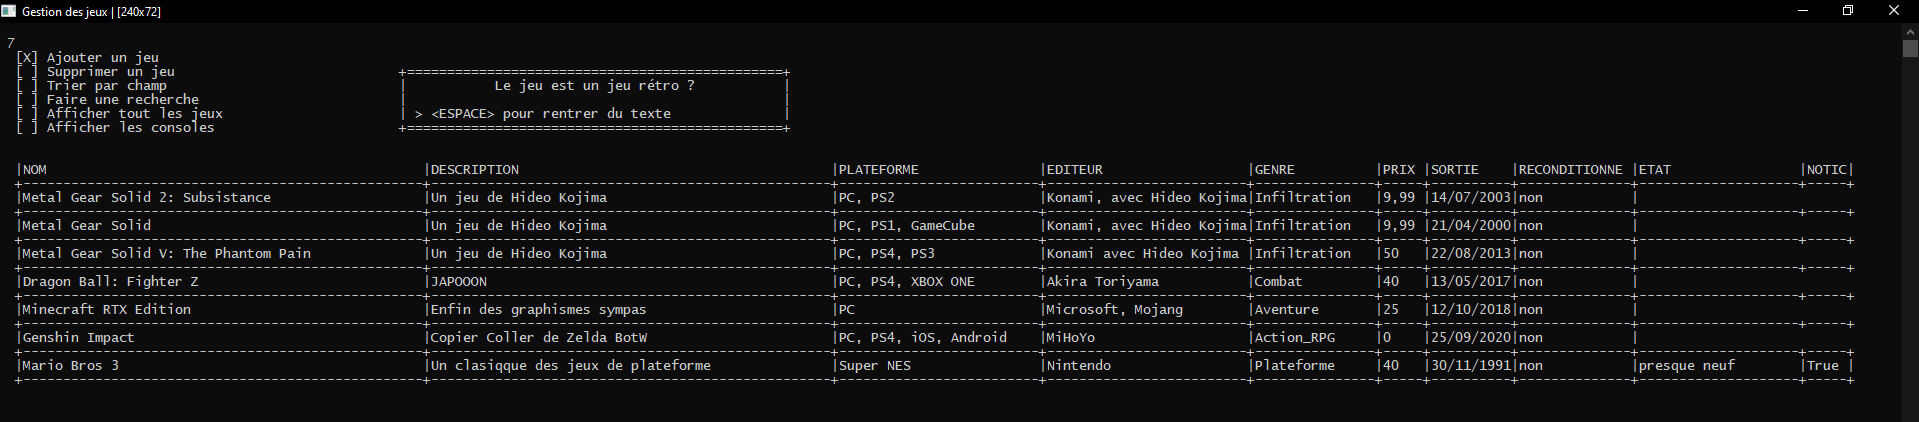
\includegraphics[scale=0.3]{screens yann/ecran_3_pre_ajout.png}
        \caption{Lors de l'ajout d'un jeu, une CLIInputWindow s'affiche pour indiquer quel paramètre entrer et dans quel format}
    \end{figure}
    
\newpage
    \begin{figure}[]
        \centering
        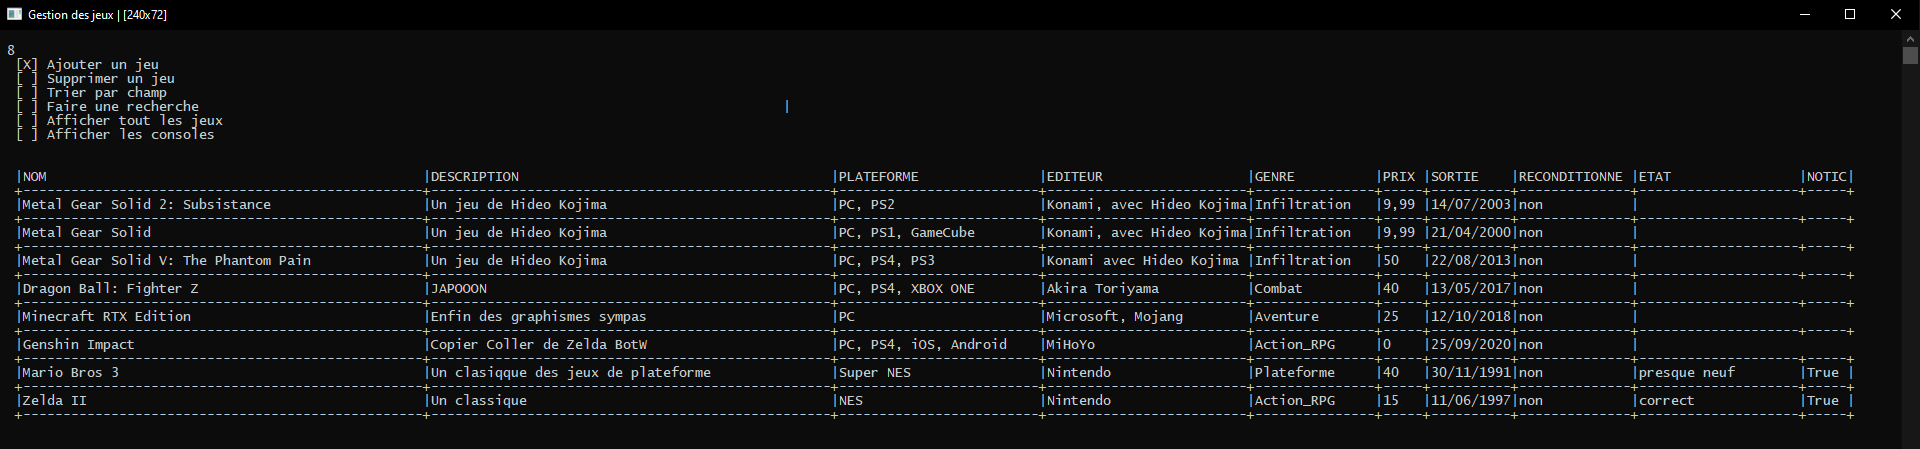
\includegraphics[scale=0.3]{screens yann/ecran_4_post_ajout.png}
        \caption{Une fois tous les paramètres rentrés, le jeu est crée et est ajouté dans la table qui sera actualisée. Ici, j'ai ajouté Zelda II.}
        
        \vspace{\baselineskip}
        
        \centering
        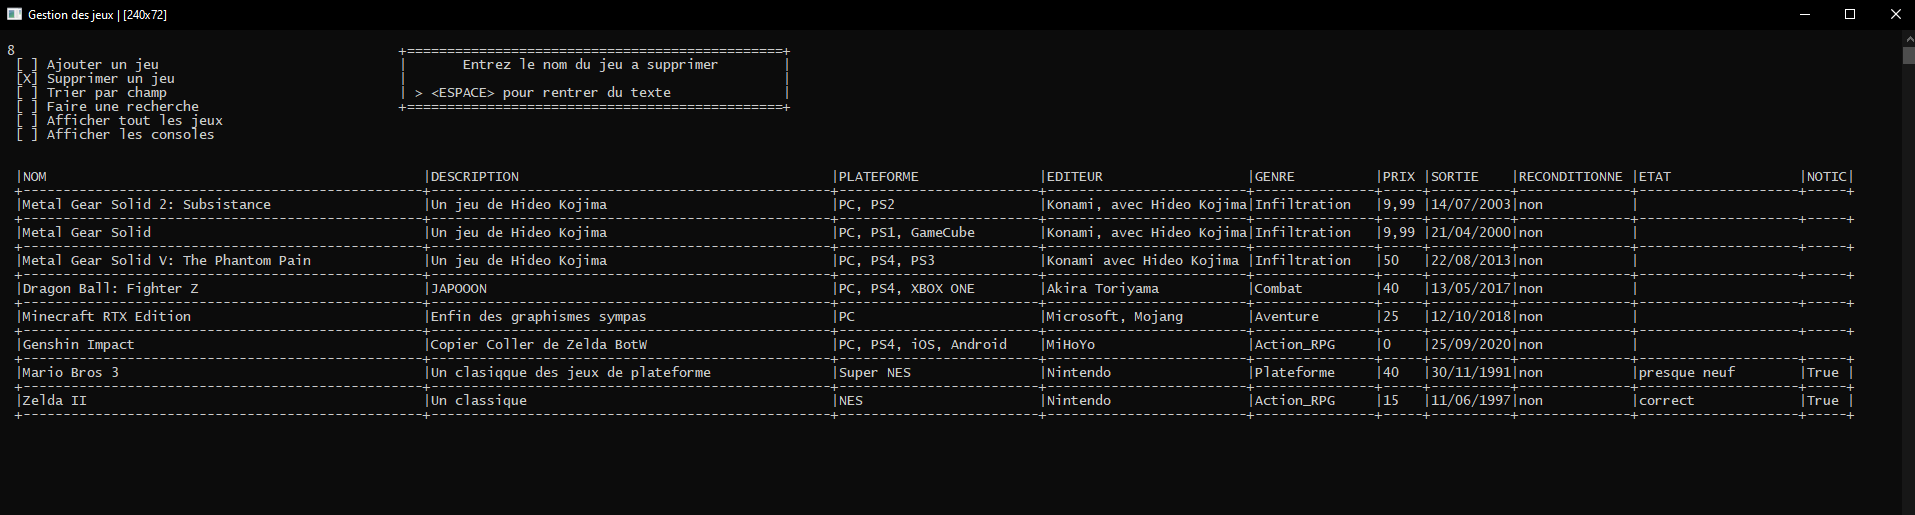
\includegraphics[scale=0.3]{screens yann/ecran_5_pre_suppression.PNG}
        \caption{Quand on veut supprimer un jeu, une CLIInputWindow s'affiche et demande le nom du jeu. Ce sera le seul paramètre demandé.}
        
        \vspace{\baselineskip}
        
        \centering
        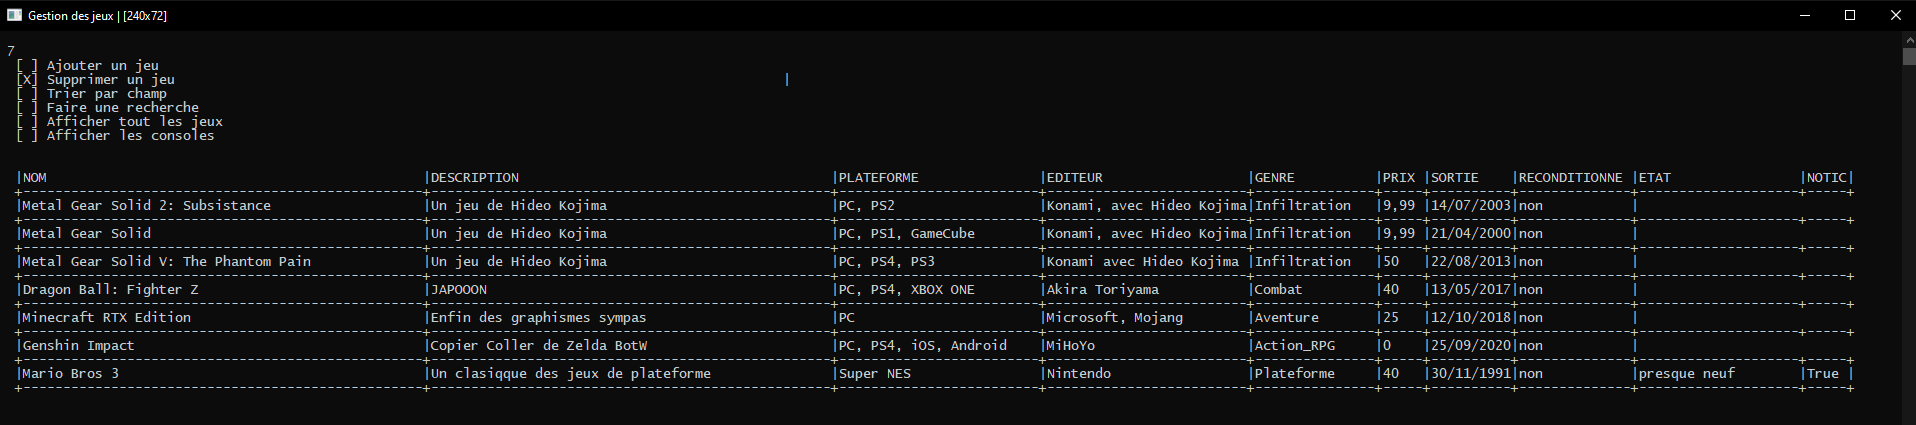
\includegraphics[scale= 0.3]{screens yann/ecran_6_post_suppression.PNG}
        \caption{Une fois le nom saisi, le jeu est supprimé et la table est mise à jour.}
    
        \vspace{\baselineskip}
        
        \centering
        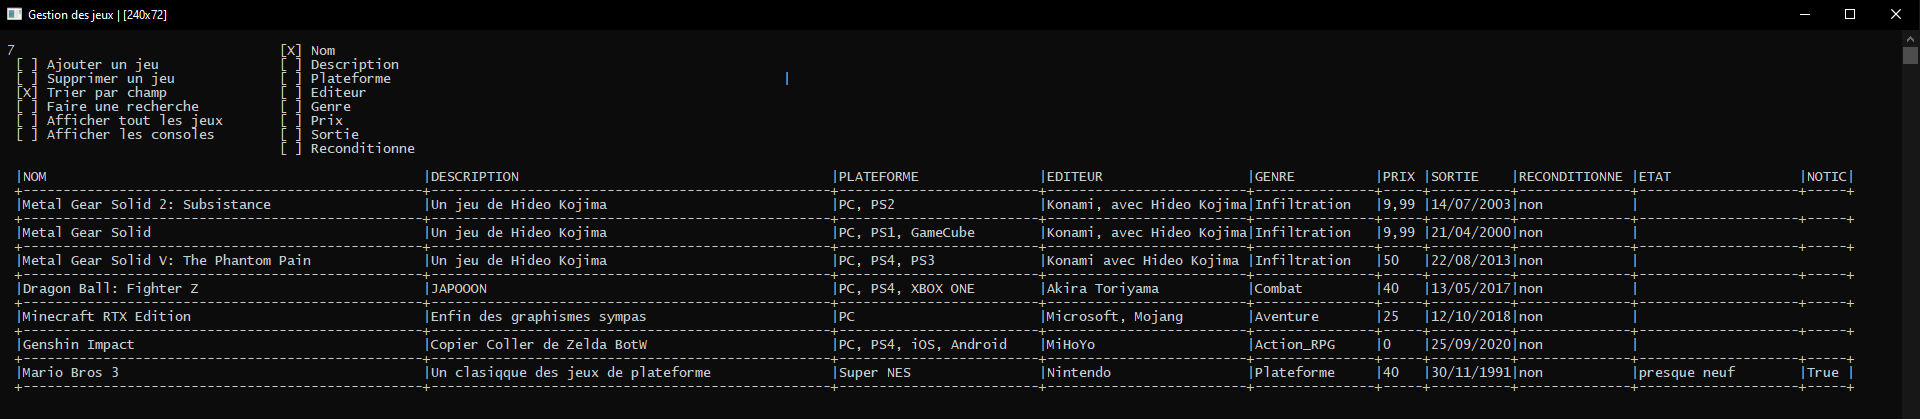
\includegraphics[scale= 0.3]{screens yann/ecran_6_pre_tri.PNG}
        \caption{Pour trier tous les jeux, il faut séléctionner la commande, puis séléctionner le champ sur lequel trier.}
    \end{figure}
    
\newpage
    \begin{figure}[]
        \centering
        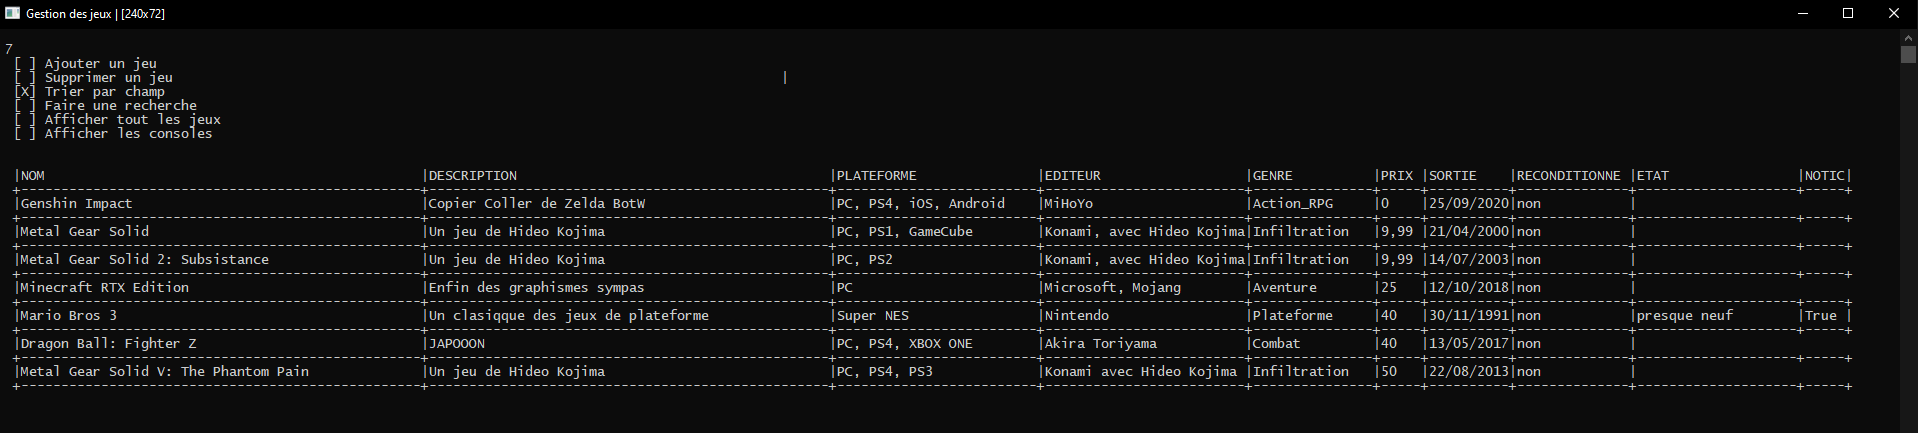
\includegraphics[scale=0.3]{screens yann/ecran_7_post_tri.PNG}
        \caption{Ici, j'ai choisi de trier les jeux par prix.}
        
        \vspace{\baselineskip}
        
        \centering
        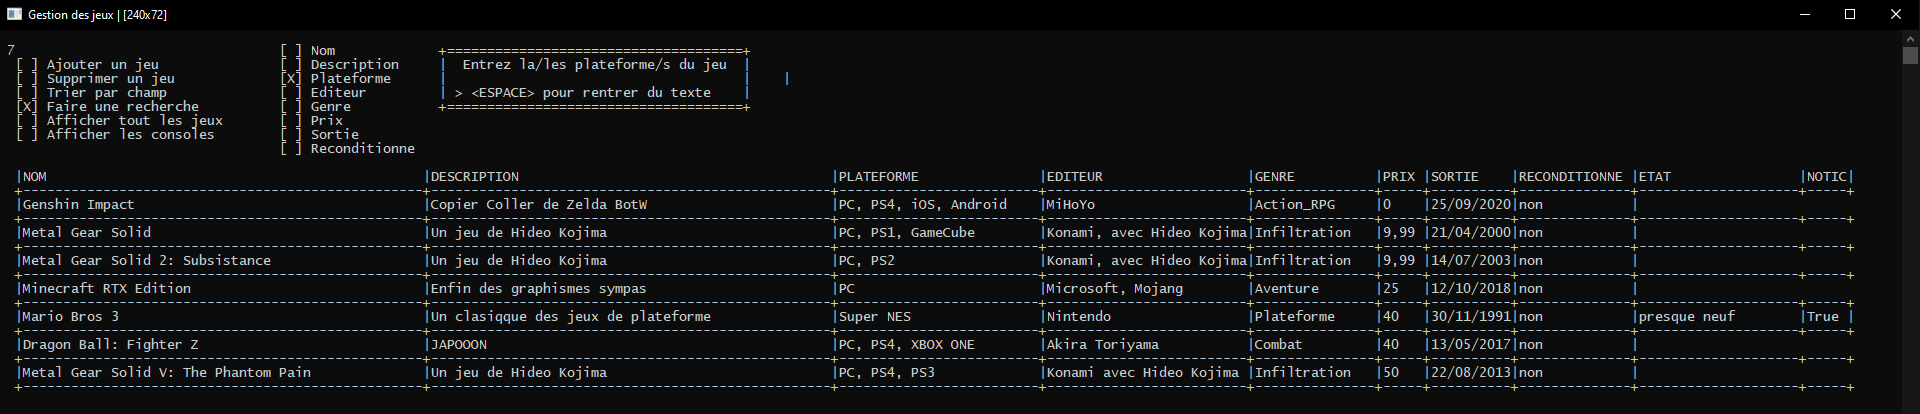
\includegraphics[scale=0.3]{screens yann/ecran_8_pre_recherche.PNG}
        \caption{La recherche fonctionne comme le tri. Séléctionnez la commande, le champ puis une CLIInputWindow demande la valeur de ce que vous voulez rechercher.}
        
        \vspace{\baselineskip}
        
        \centering
        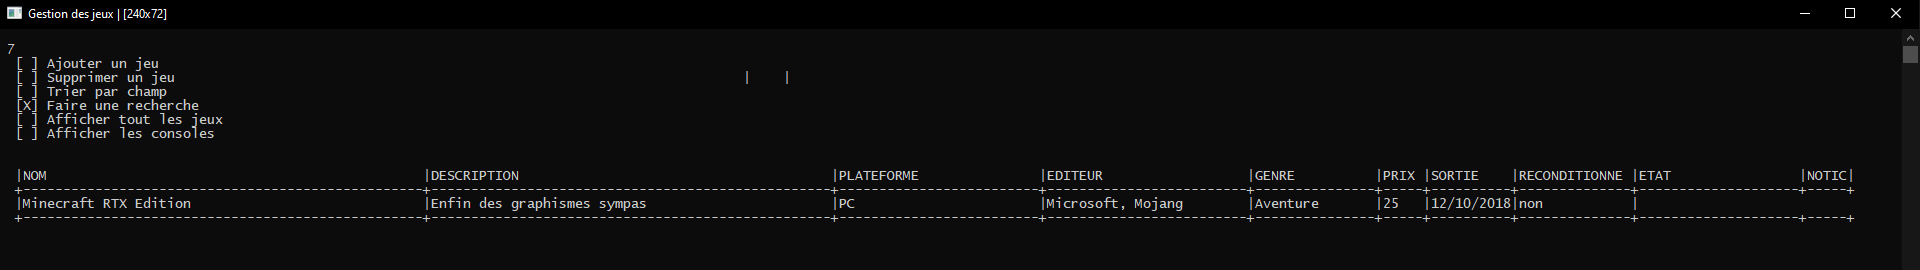
\includegraphics[scale=0.3]{screens yann/ecran_9_post_recherche.PNG}
        \caption{Le résultat d'une recherche s'affiche à la place de la table. Ici j'ai recherché les jeux n'ayant que PC comme plateforme. Pour pouvoir éxécuter une autre commande, vous devez séléctionner la commande afficher tous les jeux.}
        
        \vspace{\baselineskip}
        
        \centering
        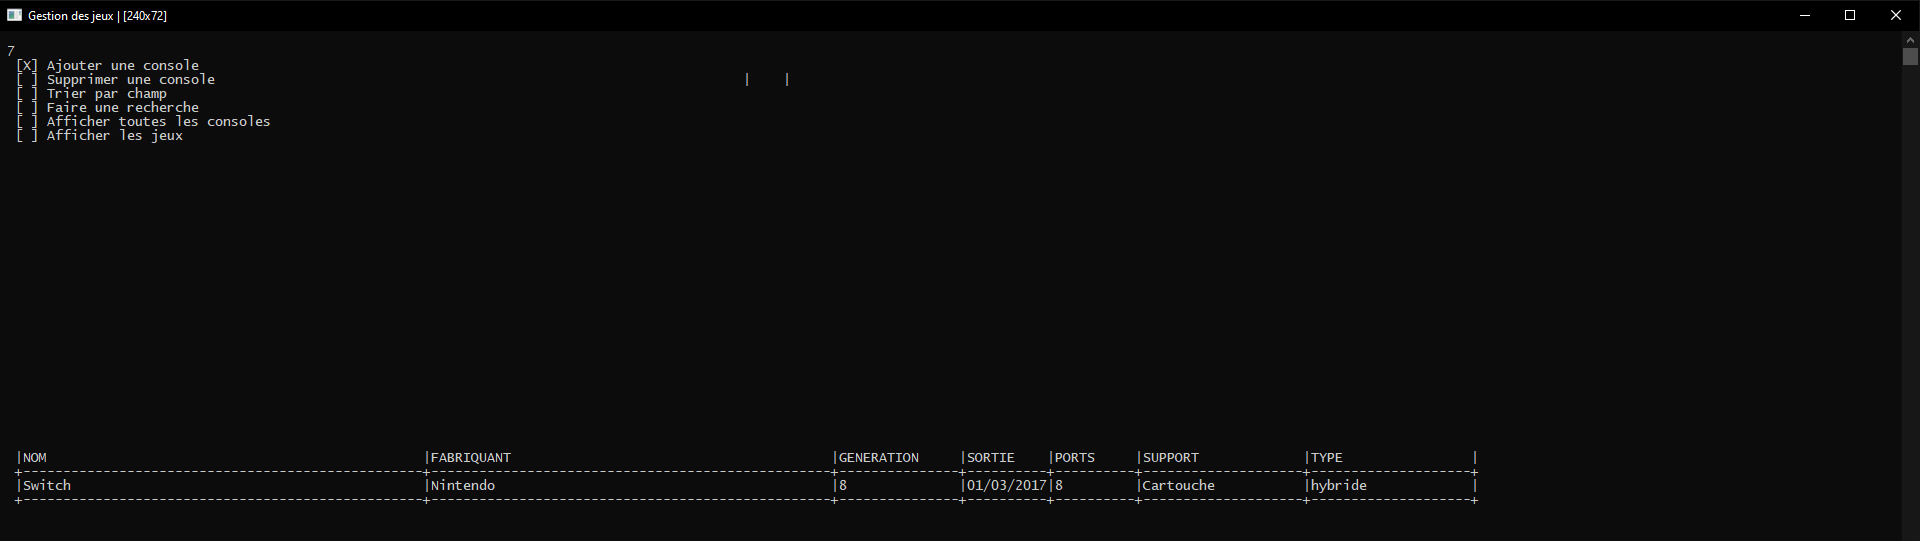
\includegraphics[scale=0.3]{screens yann/ecran_principal.PNG}
        \caption{Lorsque l'on choisit la commande afficher les consoles, le gestionnaire affiche les commandes des consoles ainsi qu'une CLITable affichant tous les jeux présents dans le catalogue. Les commandes se comportent exactement comme celles vues précédement donc nous n'allons pas en parler.}
    \end{figure}
    
\newpage
    \subsection*{2. Dépannage}
    Il peut arriver que le programme plante. Comme indiqué au dessus, une des erreurs que vous risquez le plus de rencontrer est liée à la console. Mais il y en a quelques autres qui peuvent être rencontrées. Notamment lors de la saisie des attributs pendant l'ajout, si le format n'est pas celui prévu, le programme plantera. 
    \\
    Une corruption de l'affichage peut apparaitre: du texte la il n'est sensé rien y avoir. Son origine est inconnue, si elle est constatée, effectuez une ou deux commandes pour qu'elle disparaisse.
    \\\\
    Ce sont les erreurs que nous avons rencontrées et qui sont encore présentes, dans l'attente d'un correctif.
\newpage
    \section*{IV | Panier générique d'objets}
    Pour terminer, nous allons parler du panier d'objets. Il utilise un type générique qui doit implémenter IComparable et IEquatable pour pouvoir trier le tableau et vérifier l'existence de doublons. 
    La taille maximum du tableau a été fixée à 50 éléments. Si le tableau est plein et que l'on demande l'ajout, une exeption sera envoyée. On peut donc ajouter des éléments, les supprimer, trier le tableau grâce au tri à bulles et enfin afficher le panier avec sa méthode ToString().

\end{document}